\subsection{Results}\label{sec:results}

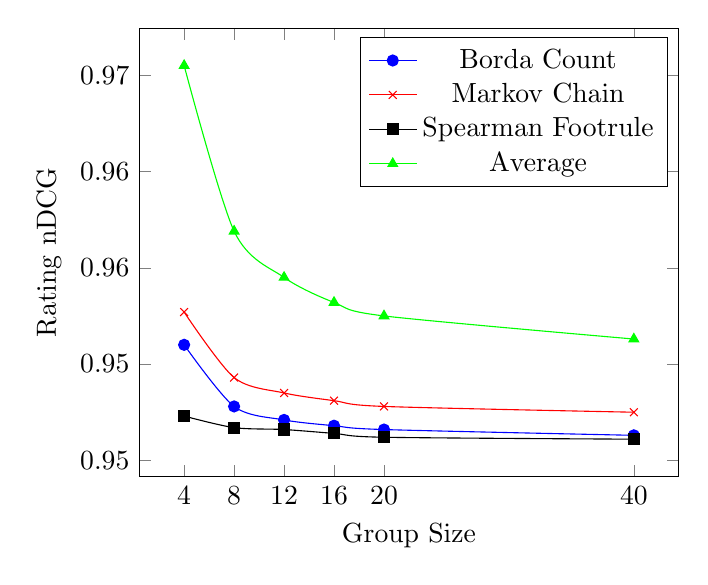
\begin{tikzpicture}
    \begin{axis}[
        xlabel=Group Size,
        ylabel=Rating nDCG,
        xtick = {4,8,12,16,20,40}]
    \addplot[smooth,mark=*,blue] plot coordinates {
        (4,0.956)
        (8,0.9528)
        (12,0.9521)
        (16,0.9518)
        (20,0.9516)
        (40,0.9513)
    };
    \addlegendentry{Borda Count}

    \addplot[smooth,color=red,mark=x] plot coordinates {
            (4,0.9577)
            (8,0.9543)
            (12,0.9535)
            (16,0.9531)
            (20,0.9528)
            (40,0.9525)
        };
    \addlegendentry{Markov Chain}
    
        \addplot[smooth,color=black,mark=square*] plot coordinates {
            (4,0.9523)
            (8,0.9517)
            (12,0.9516)
            (16,0.9514)
            (20,0.9512)
            (40,0.9511)
        };
    \addlegendentry{Spearman Footrule}
    
    \addplot[smooth,color=green,mark=triangle*] plot coordinates {
            (4,0.9705)
            (8,0.9619)
            (12,0.9595)
            (16,0.9582)
            (20,0.9575)
            (40,0.9563)
        };
    \addlegendentry{Average}
    
    \end{axis}
\end{tikzpicture}

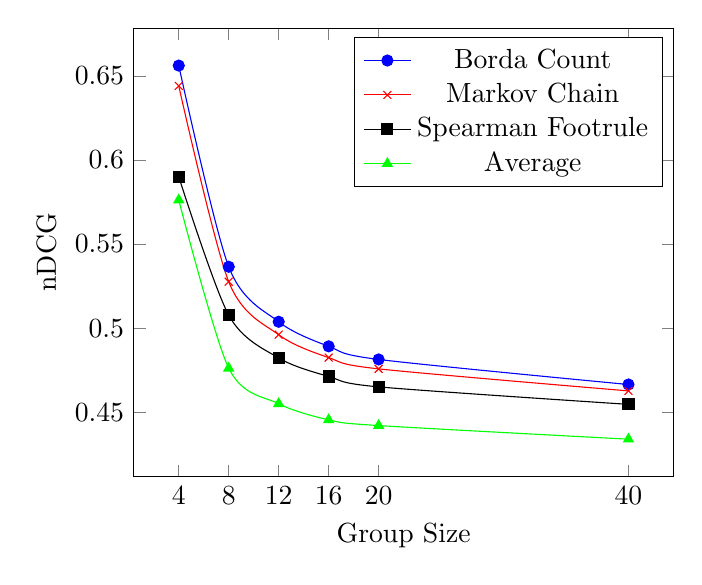
\begin{tikzpicture}
    \begin{axis}[
        xlabel=Group Size,
        ylabel=nDCG,
        xtick = {4,8,12,16,20,40}]
    \addplot[smooth,mark=*,blue] plot coordinates {
        (4,0.6561)
        (8,0.5365)
        (12,0.5038)
        (16,0.4892)
        (20,0.4814)
        (40,0.4665)
    };
    \addlegendentry{Borda Count}

    \addplot[smooth,color=red,mark=x] plot coordinates {
            (4,0.6440)
            (8,0.5276)
            (12,0.4961)
            (16,0.4825)
            (20,0.4758)
            (40,0.4627)
        };
    \addlegendentry{Markov Chain}
    
        \addplot[smooth,color=black,mark=square*] plot coordinates {
            (4,0.59)
            (8,0.5077)
            (12,0.4823)
            (16,0.4713)
            (20,0.4651)
            (40,0.4547)
        };
    \addlegendentry{Spearman Footrule}
    
    \addplot[smooth,color=green,mark=triangle*] plot coordinates {
            (4,0.5762)
            (8,0.4762)
            (12,0.4551)
            (16,0.4455)
            (20,0.4421)
            (40,0.434)
        };
    \addlegendentry{Average}
    
    \end{axis}
\end{tikzpicture}

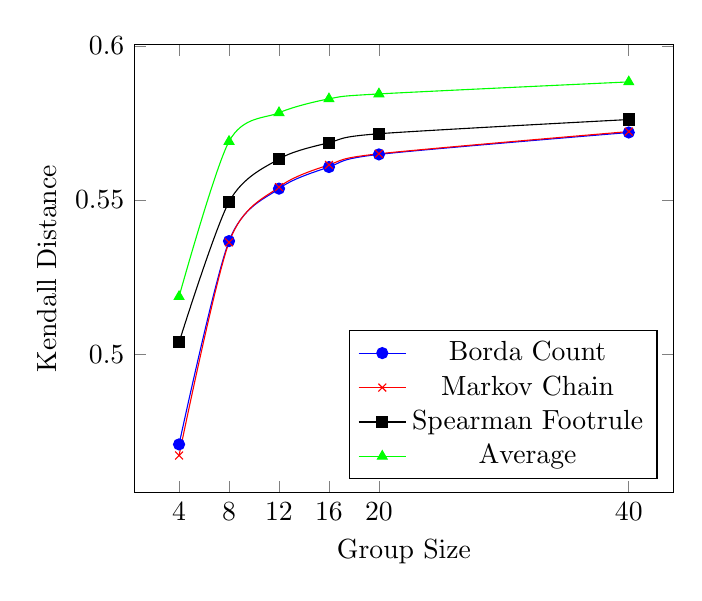
\begin{tikzpicture}
    \begin{axis}[
        xlabel=Group Size,
        ylabel=Kendall Distance,
        xtick = {4,8,12,16,20,40},
        legend pos=south east]
    \addplot[smooth,mark=*,blue] plot coordinates {
        (4,0.4708)
        (8,0.5367)
        (12,0.5537)
        (16,0.5607)
        (20,0.5648)
        (40,0.5719)
    };
    \addlegendentry{Borda Count}

    \addplot[smooth,color=red,mark=x] plot coordinates {
            (4,0.4672)
            (8,0.5363)
            (12,0.5542)
            (16,0.5614)
            (20,0.565)
            (40,0.5722)
        };
    \addlegendentry{Markov Chain}
    
        \addplot[smooth,color=black,mark=square*] plot coordinates {
            (4,0.5039)
            (8,0.5494)
            (12,0.5633)
            (16,0.5686)
            (20,0.5715)
            (40,0.5761)
        };
    \addlegendentry{Spearman Footrule}
    
    \addplot[smooth,color=green,mark=triangle*] plot coordinates {
            (4,0.5187)
            (8,0.569)
            (12,0.5783)
            (16,0.5828)
            (20,0.5844)
            (40,0.5883)
        };
    \addlegendentry{Average}
    
    \end{axis}
\end{tikzpicture}

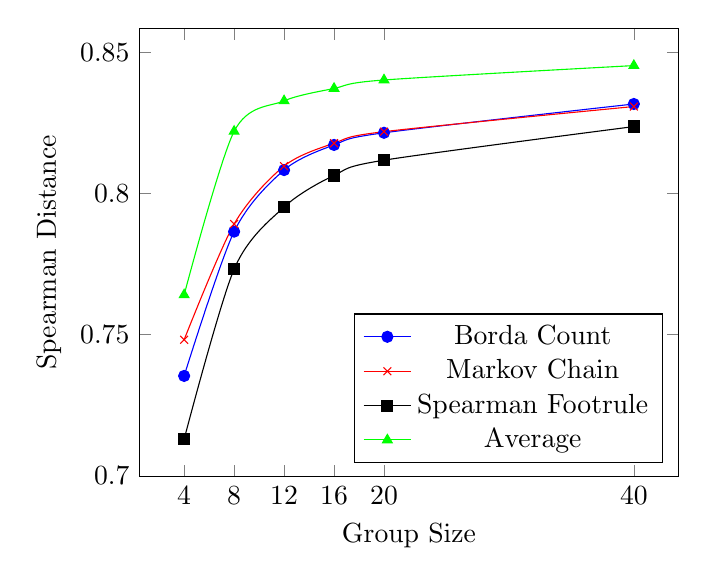
\begin{tikzpicture}
    \begin{axis}[
        xlabel=Group Size,
        ylabel=Spearman Distance,
        xtick = {4,8,12,16,20,40},
        legend pos=south east]
    \addplot[smooth,mark=*,blue] plot coordinates {
        (4,0.7354)
        (8,0.7865)
        (12,0.8083)
        (16,0.8172)
        (20,0.8215)
        (40,0.8317)
    };
    \addlegendentry{Borda Count}

    \addplot[smooth,color=red,mark=x] plot coordinates {
            (4,0.7482)
            (8,0.7892)
            (12,0.8097)
            (16,0.8178)
            (20,0.8219)
            (40,0.8308)
        };
    \addlegendentry{Markov Chain}
    
        \addplot[smooth,color=black,mark=square*] plot coordinates {
            (4,0.7130)
            (8,0.7732)
            (12,0.7952)
            (16,0.8064)
            (20,0.8118)
            (40,0.8237)
        };
    \addlegendentry{Spearman Footrule}
    
    \addplot[smooth,color=green,mark=triangle*] plot coordinates {
            (4,0.7641)
            (8,0.822)
            (12,0.8328)
            (16,0.8372)
            (20,0.8402)
            (40,0.8453)
        };
    \addlegendentry{Average}
    
    \end{axis}
\end{tikzpicture}